\chapter{Introduction}
%\epigraph{\textit{TBD quote about science or something \\ cool and poetic}}{TBD Person who said quote}
\label{chap:intro}
In this thesis we investigate the large-scale configuration and dynamics of Saturn's magnetosphere, using \textit{in situ} data and computer models. But first, we must consider the fundamental physics concepts that allow us to understand Saturn's magnetosphere, and the language we will use to describe it. 

Saturn's magnetosphere comprises magnetic fields, electric fields and \textit{plasma}. \textit{Plasma} is considered the fourth state of matter after solid, liquid, and gas, and is formed of a gas that has been ionised, such that the atoms have been split up into negatively charged electrons and positively charged ions. Unlike neutral particles, charged particles are influenced by electric and magnetic fields, and this fundamentally determines how plasma behaves differently to other neutral states of matter. We therefore start this chapter with a discussion of how charged particles are affected by electromagnetic forces, and how we can understand these effects by considering the plasma as a bulk fluid. We then discuss the nature of the magnetised plasmas we encounter in space, moving outwards through the solar system from the Sun to Earth, Jupiter and finally Saturn. We provide details for the construction of a force-balance model of Saturn's \textit{magnetodisc}, which is used throughout this thesis as a tool to explore the behaviour of Saturn's magnetosphere. We finish the chapter with a summary of the open questions in this area of research, some of whic h this thesis plans to address.

\section{Physics of Magnetised Plasmas}
\subsection{Forces on an Individual Charged Particle}\label{intro:sec:singleparticle}
We begin with Maxwell's equations of electromagnetism. These are:
\begin{equation}
\nabla \times \boldsymbol{E} = -\frac{\partial \boldsymbol{B}}{\partial t}
\end{equation}
\begin{equation}\label{intro:eq:amperemaxwell}
\nabla \times \boldsymbol{B} = \mu_0 \boldsymbol{J} + \frac{1}{c^2}\frac{\partial \boldsymbol{E}}{\partial t}
\end{equation}
\begin{equation}
\nabla \cdot \boldsymbol{E} = \frac{\rho_q}{\epsilon_0} 
\end{equation}
\begin{equation}\label{intro:eq:nomonopoles}
\nabla \cdot \boldsymbol{B} = 0.
\end{equation}
These equations govern how electric ($\boldsymbol{E}$) and magnetic ($\boldsymbol{B}$) fields vary over time $t$ and through space. $\boldsymbol{J}$ is the current density, $\rho_q$ is the charge density, $c^2 = 1/\mu_0 \epsilon_0$ is the square of the speed of light, and $\mu_0$ and $\epsilon_0$ are the constants known as the permeability and permittivity of free space. Together with the Lorentz force law, we can use these equations to understand how a charged particles interact with electric and magnetic fields. The Lorentz force is given by 
\begin{equation}\label{intro:eq:lorentz}
\boldsymbol{F}_\mathrm{L} = q(\boldsymbol{E} + \boldsymbol{v} \times \boldsymbol{B}),
\end{equation}
where $q$ is the charge of the particle and $\boldsymbol{v}$ its velocity. In the absence of an electric field, and with a uniform magnetic field, it can be shown that this Lorentz force causes the charged particle to gyrate around the magnetic field direction, with angular frequency
\begin{equation}
\Omega_c = \frac{|q|B}{m}
\end{equation}
known as the cyclotron frequency, where $m$ is the mass of the particle and $B$ is the magnitude of the magnetic field. From equation~\ref{intro:eq:lorentz}  with $\boldsymbol{E}=0$, positively charged particles gyrate in a left-handed sense around the magnetic field, and negatively charged particles gyrate in a right-handed sense. The radius of this orbit is given by the gyroradius, or Larmor radius,
\begin{equation}
r_\mathrm{L} = \frac{v_\perp}{\Omega_c} = \frac{mv_\perp}{|q|B}
\end{equation}
where $\perp$ and later $\parallel$ subscripts refer to components perpendicular and parallel to the magnetic field. $r_\mathrm{L}$ is generally larger for ions (which are more massive than electrons), and for particles with higher energy (and so higher $v_\perp$). Note that the Lorentz force acts perpendicular to the magnetic field by definition, and so the motion of charged particles \textit{parallel} to the magnetic field is not affected by $\boldsymbol{B}$; charged particles are thus free to move up and down along magnetic field lines, in the absence of other forces.

In a spatially non-uniform magnetic field, a particle will not only gyrate around a magnetic field line, but the guiding centre of its gyratory motion will also drift, depending on the variation of the magnetic field. The velocity of this guiding-centre motion is given by the gradient drift velocity
\begin{equation}
\boldsymbol{v}_\mathrm{g} = \frac{mv_\perp\boldsymbol{B}\times\nabla B}{2qB^3}
\end{equation}
and is therefore in a direction perpendicular to both the magnetic field direction and the gradient of the magnetic field magnitude. In an approximately dipolar magnetic field, e.g. at Saturn, the magnetic field strength decreases with radial distance, and so $\nabla B$ is oriented radially inwards, while the magnetic field $\boldsymbol{B}$ is oriented downwards near the equator (or upwards at other magnetised planets, such as Earth and Mercury). At Saturn, this has the net effect of causing positively charged ions to drift eastwards, and negatively charged electrons to drift westwards, which sets up a net flow of charge (i.e. current) eastwards, in the direction of planetary rotation.

In a dipolar magnetic field, the magnetic field lines are also curved, and so a charged particle gyrating and also moving freely along a magnetic field line will feel a centrifugal force. This force also induces a drift in the guiding centre of the charged particle's orbit, given by the curvature drift velocity
\begin{equation}
\boldsymbol{v}_\mathrm{c} = \frac{mv_\parallel^2~\boldsymbol{r}_\mathrm{c}\times\boldsymbol{B}}{qB^2r_\mathrm{c}^2}
\end{equation}
where $\boldsymbol{r}_\mathrm{c}$ is the radius of curvature vector for the magnetic field line, defined as pointing radially outwards from the centre of curvature to the particle. (As an example, for a dipole magnetic field $r_\mathrm{c}= r/3$ at the magnetic equator, where $r$ is the radial distance from the origin.) This therefore has the same effect as the gradient drift force, with ions drifting eastwards and electrons drifting westwards, resulting in a net current in the direction of planetary rotation. 

For a general external force $\boldsymbol{F}$ the guiding-centre drift associated with that force is given by
\begin{equation}\label{intro:eq:vf}
\boldsymbol{v}_\mathrm{F} = \frac{\boldsymbol{F}\times\boldsymbol{B}}{qB^2}.
\end{equation}

For the case $\boldsymbol{F} = q\boldsymbol{E}$, the force exerted by an electric field $\boldsymbol{E}$, then the $q$ term on the denominator of equation~(\ref{intro:eq:vf}) cancels, and $\boldsymbol{v}_\mathrm{F}$ is independent of $q$ such that both electrons and ions drift in the same direction.

Finally, it is important to consider the phenomenon of magnetic mirroring of charged particles, as this dynamical effect is common in the approximately dipolar magnetic fields of magnetised planets. The magnetic moment $\mu_\mathrm{m}$ of a charged particle gyrating in a circular orbit around a magnetic field with gyroradius $r_\mathrm{L}$, can be written as
\begin{equation}
\mu_\mathrm{m} = \frac{mv_\perp^2}{2B}
\end{equation}
from the definition $\mu = IA$, with $I = q\Omega_\mathrm{c}/2\pi$ and $A = \pi r_\mathrm{L}^2$. For a slowly varying magnetic field, this quantity is conserved and is known as the \textit{first adiabatic invariant}. A consequence of this is that as a particle gyrates along a magnetic field line towards a region where the magnetic field strength increases (e.g. polar regions of a dipole magnetic field), the particle's perpendicular velocity $v_\perp$ must also increase. Without an external electric field to do work on the particle, the total energy of the particle $\frac{1}{2}m(v_\perp^2+v_\parallel^2)$ must remain constant, and so an increase in $v_\perp$ coincides with a decrease in $v_\parallel$, until $v_\parallel$ reaches zero and the particle is `reflected' back along the magnetic field line in the opposite direction. That is, the motion of the guiding centre of the particle motion reverses direction. This phenomenon causes charged particles to `bounce' up and down along dipolar magnetic field lines, reflecting near the poles where the magnetic field strength acquires a value large enough to reverse the guiding centre motion. 

Therefore, charged particles in a planetary dipole magnetic field simultaneously gyrate around the magnetic field lines, bounce up and down along them, and drift azimuthally around the planet in a direction depending on their charge.

\subsection{Forces on a Collective Plasma}
% From Space notes eq 2.35 etc. can explain what rho, J is for the electron and ion population seperatly if necessary 
Considering the motion of individual charged particles can only get us so far when trying to understand the global dynamics of large-scale plasma structures, such as planetary magnetospheres. It can be helpful to describe the plasma as a single fluid, with a bulk plasma flow velocity $\boldsymbol{u}$. This approach is known as single fluid magnetohydrodynamics (MHD), and the \textit{momentum equation} for the plasma fluid is given by
\begin{equation}\label{intro:eq:momentum}
\rho\frac{d\boldsymbol{u}}{dt} = \rho_\mathrm{q}\boldsymbol{E} + \boldsymbol{J}\times\boldsymbol{B} - \nabla P + \rho \boldsymbol{g}
\end{equation}
where $\rho$ is the mass density of the plasma, P is the plasma pressure (assumed to be isotropic), and $\boldsymbol{g}$ is the acceleration due to gravity. The first terms on the right hand side correspond to the Lorentz force terms given in equation~\ref{intro:eq:lorentz} for the bulk plasma. However if we assume quasi-neutrality, such that the density of ions and the density of electrons in the plasma are approximately equal, then $\rho_\mathrm{q}$ is negligible and we can ignore the effect of the electric field $\boldsymbol{E}$. This is appropriate when considering plasmas over large temporal or spatial scales, as the individual charged particles quickly adjust to remove any charge imbalance caused by local density variations. Similarly in most space plasmas we can neglect the gravitational term as being insignificant compared to other terms.

This leaves the plasma pressure gradient force and the $\boldsymbol{J}\times\boldsymbol{B}$ force as the dominant forces on the magnetised plasma. To understand the effect of the $\boldsymbol{J}\times\boldsymbol{B}$ force in particular on the plasma, it is helpful to consider the case where plasma flows are significantly slower than the speed of light, which is appropriate for space plasmas considered in this thesis. In this case, we can neglect the second `displacement current' term in the Maxwell's equation known as the Amp\`ere-Maxwell relation (equation~\ref{intro:eq:amperemaxwell}), and so this simplifies to 
\begin{equation}\label{intro:eq:ampere}
\nabla \times \boldsymbol{B} = \mu_0 \boldsymbol{J} 
\end{equation}
known as Amp\`ere's Law. This allows the $\boldsymbol{J}\times\boldsymbol{B}$ force to be rewritten as
\begin{equation}\label{intro:eq:bpressuretension}
\boldsymbol{J}\times\boldsymbol{B} = -\nabla\left(\frac{B^2}{2\mu_0}\right)+\frac{1}{\mu_0}(\boldsymbol{B}\cdot\nabla)\boldsymbol{B}.
\end{equation}
The first term on the right hand side corresponds to a magnetic pressure gradient force, with magnetic pressure $P_\mathrm{B} = B^2/2\mu_0$. The second term on the right hand side corresponds to the magnetic tension force. The component of this force perpendicular to the magnetic field direction, known as the curvature force, acts to `straighten' bent field lines, akin to the restoring force on a bent elastic band, and scales with the magnetic field strength and radius of curvature as $B^2/r_\mathrm{c}$. The component of this force parallel to the magnetic field lines cancels out exactly with the parallel component of the magnetic pressure gradient force, as the total $\boldsymbol{J}\times\boldsymbol{B}$ force must act perpendicular to the magnetic field by definition.

We will return to these concepts of magnetic pressure and tension forces, and discuss force balance in the plasma in these terms throughout this thesis.

\subsection{The Frozen-in Field Theorem}\label{intro:sec:frozenin}
%could remove length/time scales because kind of already assumed this when assumed quasineutrality and flow much slower than c
If we make a few more simplifying assumptions about the nature of our plasma, we have conditions for \textit{ideal MHD}. In particular we assume the plasma conditions do not vary on length scales and time scales smaller than the particle gyroradius nor the associated gyroperiod. We also assume the conductivity of the plasma is sufficiently high that we can neglect Joule heating, resistivity and collisions between particles, which is appropriate for the collisionless space plasmas that we consider in this thesis. This leads us to the idealised Ohm's Law,
\begin{equation}\label{intro:eq:ohms}
\boldsymbol{E} + \boldsymbol{u} \times \boldsymbol{B} = 0
\end{equation}
An important mathematical consequence of this is the \textit{frozen-in field theorem}. This powerful theorem states, under the conditions as described above, that the plasma and the magnetic field are `frozen in' to each other and move together. From equation~\ref{intro:eq:ohms} it can be shown that if a magnetic field threads through two plasma fluid elements, the field will continue to connect them even as the elements move and change shape and size. This also means that two different plasma populations embedded with different magnetic fields cannot mix.

This theorem is instructive in intuitively understanding the behaviour of many space plasmas, including planetary magnetospheres. To determine whether the plasma approximately follows the magnetic field, or the magnetic field approximately follows the plasma, it is useful to consider the quantity plasma $\beta$, defined as
\begin{equation}
\beta = \frac{P}{B^2/2\mu_0}
\end{equation}
the ratio of the plasma to magnetic pressure. In high $\beta$ ($>>1$) regimes, the plasma dominates, and the magnetic field that threads the plasma is convected along with the plasma flow. In low $\beta<1$ regimes, the opposite is the case, and the plasma is locked into the moving magnetic field. Both regimes are found in space plasmas (discussed in the rest of this chapter), and we will encounter both regimes in our study of Saturn's magnetosphere in this thesis. In particular we will often refer to `flux tubes' of plasma in Saturn's magnetosphere, which are volumes of plasma mapped out by the planetary dipole magnetic field lines, and which obey this frozen-in condition.

When the magnetic field varies on length scales comparable to the gyroradius of the individual plasma particles, ideal MHD breaks down and the frozen-in field theorem no longer holds. In this case, we observe a phenomenon known as \textit{reconnection}, where magnetic field lines that were previously separated by different plasma populations are forced close enough together that they reconnect. This can cause an explosive release of plasma along the newly reconnected magnetic field lines, and a reconfiguration of the magnetic field. This is a fundamental process planetary magnetospheres, as discussed in more detail in Section~\ref{intro:sec:dynamics}. 
%Once written can add references to this section throughout, e.g. in corona movement explanation, force balance, magnetic tension force.

\subsection{Plasma Waves}
Many different types of waves can be set up in magnetospheric plasma populations. If we assume these waves are small in amplitude and thus only cause first-order perturbations to the background plasma properties (represented by the subscript 0 in the following equations), then we can use MHD to characterise their propagation speeds. The speed of sound in the plasma is defined as
\begin{equation}
c_\mathrm{s} = \sqrt{\frac{\gamma P_0}{\rho_0}},
\end{equation}
as for a classical gas, where $\gamma$ is the ratio of specific heats. If we assume the plasma is incompressible, and \textit{cold} such that $P_0 = c_\mathrm{s} = 0$, the MHD relations we have discussed can be used to derive the dispersion relation for the plasma:
\begin{equation}\label{intro:eq:colddispersion}
\omega^2 = k^2{v}_\mathrm{A}^2\cos^2{\theta}
\end{equation}
where $\omega$ is the wave angular frequency, $k$ is the wave number and $\theta$ is the angle between the wave propagation direction and the background magnetic field direction. $v_\mathrm{A}$ is a characteristic speed known as the \textit{Alfv\'en speed},
\begin{equation}
v_\mathrm{A} = \frac{B_0}{\sqrt{\mu_0\rho_0}}.
\end{equation}
Physically, oscillations in the magnetic field travel along the background magnetic field direction at this speed, analogous to waves propagating on a massive string. As shown by equation~\ref{intro:eq:colddispersion}, the phase velocity depends on $\theta$, and is maximum (equal to $v_\mathrm{A}$) for propagation parallel to the magnetic field, and minimum (0) for propagation perpendicular to the field. 

If instead we consider a \textit{warm} plasma and include the effect of plasma pressure, this dispersion relation becomes
\begin{equation}
\frac{\omega^2}{k^2} = \frac{1}{2}\left(c_\mathrm{s}^2+v_\mathrm{A}^2\pm\sqrt{(c_\mathrm{s}^2+v_\mathrm{A}^2)^2-4c_\mathrm{s}^2v_\mathrm{A}^2\cos^2\theta}\right)
\end{equation}
where the $\pm$ introduces two different wave modes, known as the \textit{fast} and \textit{slow} modes. While this dispersion relation may seem complicated, interesting results fall out when the parallel ($\cos\theta = 1$) and perpendicular ($\cos\theta = 0$) propagation cases are considered separately. In the limit of parallel propagation, the two wave modes propagate at the Alfv\'en speed $v_\mathrm{A}$ and the sound speed $c_\mathrm{s}$ respectively. For low $\beta$ plasmas, $c_\mathrm{s}<v_\mathrm{A}$ and so $v_\mathrm{A}$ is considered the \textit{fast} mode, while the opposite is the case for high $\beta$ plasmas. In the limit of perpendicular propagation, the \textit{slow} mode vanishes to zero, and the \textit{fast} mode propagates at the characteristic speed known as the \textit{magnetosonic speed} $c_\mathrm{ms}$,
\begin{equation}
c_\mathrm{ms} = \sqrt{v_\mathrm{A}^2+c_\mathrm{s}^2}.
\end{equation}

Other types of waves can also be set up in magnetised plasmas, depending on the conditions. However for the magnetospheric plasma environments we discuss in this thesis, an understanding of the Alfv\'en, sound and magnetosonic speeds is sufficient.
% \textit{Fast} mode waves arise when the variations in the magnetic and plasma pressures are in phase, and \textit{slow} mode waves arise when the pressures vary in antiphase. - is it necessary to include this?

\section{The Solar Wind} \label{intro:sec:solarwind}
The corona is the uppermost atmospheric layer of the Sun, and is composed mainly of ionised hydrogen (i.e. protons and electrons), with approximately $4\%$ ionised helium \citep{robbins1970}. This layer is heated from below by fusion processes in the deep interior, and other processes not yet fully understood, to extremely high temperatures of ${\sim}10^6\si{K}$ \citep{warren2009}. Above, the corona is surrounded by relatively empty space, and thus experiences a large thermal pressure gradient force directed radially outwards. This means that a significant fraction of the coronal plasma is energetic enough to escape the Sun's strong gravitational field, and thus streams radially outwards from the Sun through space at high speeds. This plasma flow is known as the solar wind.

The properties of the solar wind vary on many timescales, however it is still useful to consider the typical properties. The typical solar wind speed is around $\SI{450}{kms^{-1}}$ throughout the solar system, well above the local speed of sound. The particle number density falls approximately as $r^{-2}$ (the inverse square of radial distance from the Sun) in line with conservation of particle flux through an expanding spherical surface, with density from around $\SI{7}{cm^{-3}}$ at the orbit of Earth (\SI{1}{AU}) to \SI{0.07}{cm^{-3}} at the orbit of Saturn (\SI{9.6}{AU}) (where \SI{1}{AU} = \SI{1.496e8}{km}) \citep{bagenal2014} . Near the solar surface, the strong and complex magnetic field of the Sun dominates the plasma, in line with the frozen-in field theorem for low $\beta$ plasmas, and so generates phenomena such as coronal loops. However, further away from the Sun, beyond a few tens of solar radii, the magnetic field strength decreases with radial distance such that $\beta$ increases and the remnant magnetic field becomes frozen-in to the moving  solar wind plasma \citep{russell2016}. The magnetic field is therefore carried outwards into space by the flowing plasma, where it is known as the interplanetary magnetic field (IMF). The radial outflow of the solar wind, combined with the ${\sim}25$ day rotation period of the Sun, produce a spiral-like distribution of magnetised plasma in the Sun's equatorial plane which extends throughout the solar system, known as the \textit{Parker Spiral} \citep{parker1958}. This structure influences the typical orientation of the interplanetary magnetic field observed at each planet, from approximately radial at the orbit of Mercury, to approximately perpendicular to the radial flow at the orbit of Saturn. Figure~\ref{intro:fig:parkerspiral} shows a diagram of this phenomenon. The orientation of the IMF has consequences for the interaction between the solar wind and the planet, as discussed in future sections.

\begin{figure}
\centering
\noindent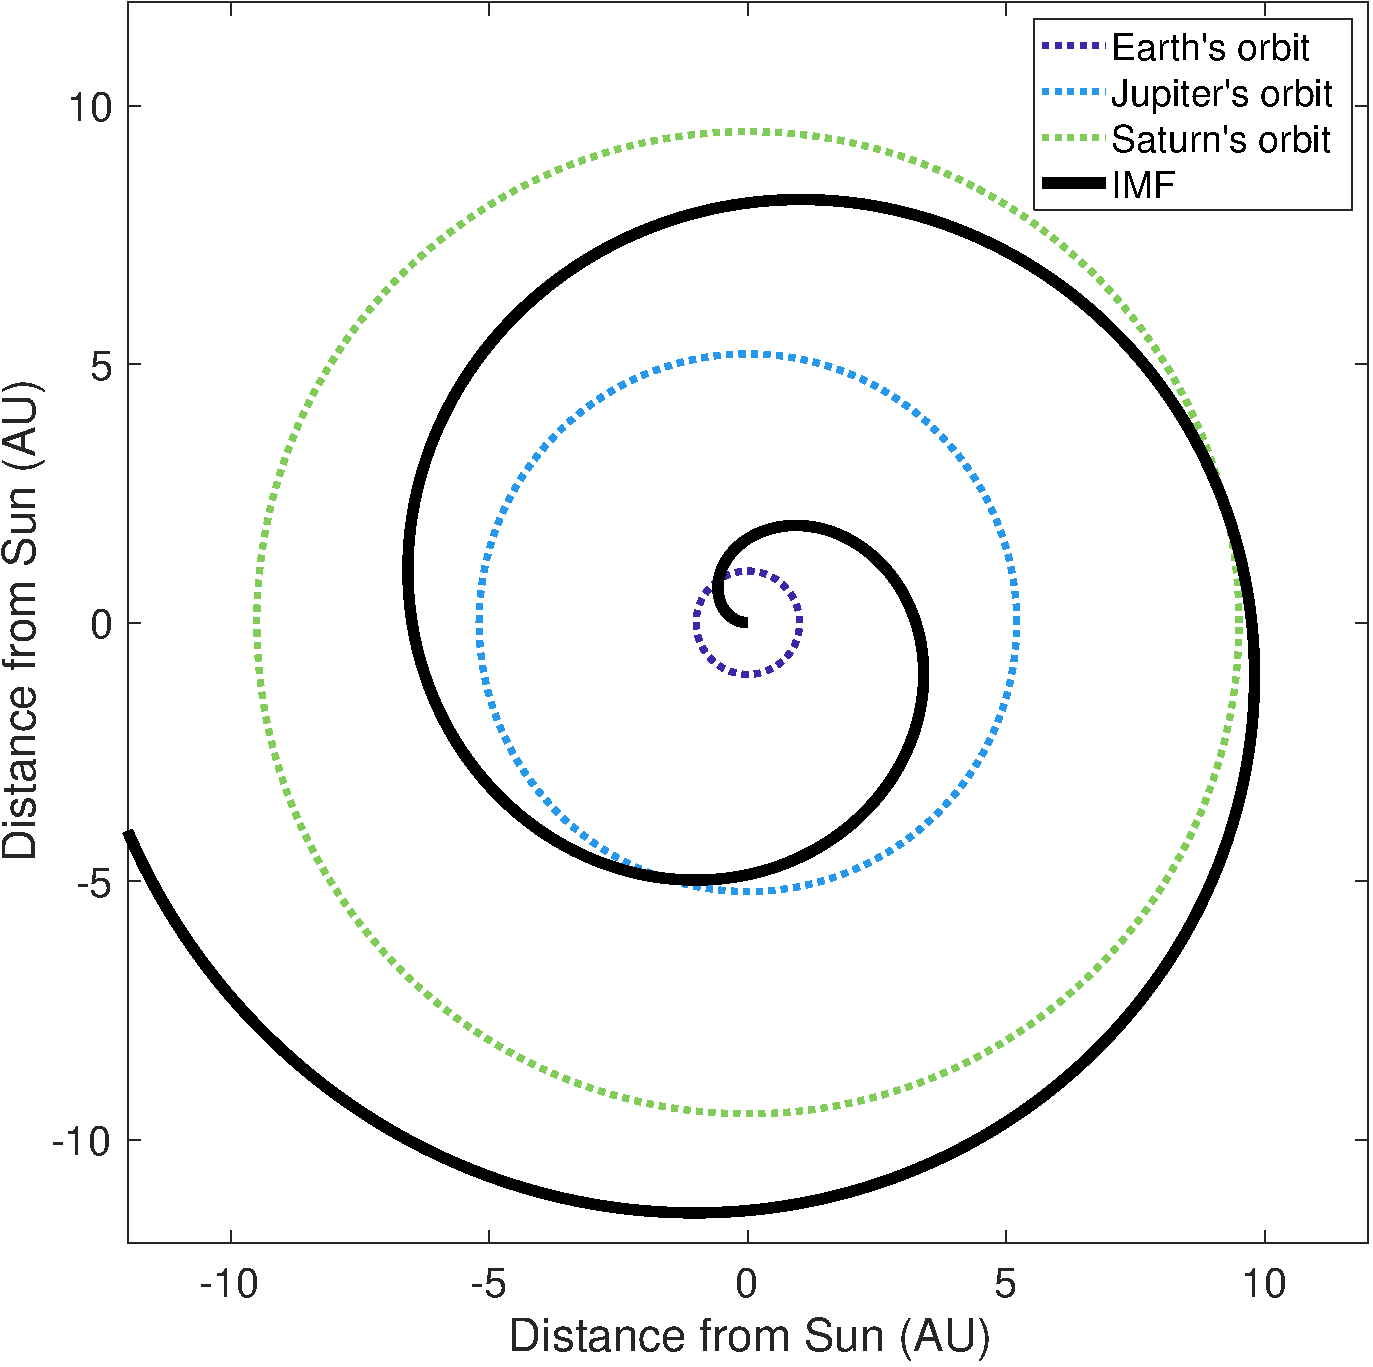
\includegraphics[width=0.6\textwidth]{intro/parkerspiral.pdf}
\caption[Diagram of the Parker Spiral throughout the solar system.]{Diagram showing how the Parker Spiral affects the orientation of the IMF (interplanetary magnetic field) in the equatorial plane throughout the solar system. The orbits of different planets are shown by the coloured dotted lines.}
\label{intro:fig:parkerspiral}
\end{figure}

On top of this rotating structure, the properties of the solar wind vary on timescales ranging from minutes to years. At the shorter end of the time spectrum, coronal mass ejections (CMEs) are dynamic outflows of dense, coronal material that occur due to dramatic reconfiguration of the coronal magnetic field. These typically form over days and may reach speeds as high as several thousand $\si{km s^{-1}}$ as they accelerate through the inner solar system. Their movements are associated with regions of enhanced density and magnetic field strength compared to the ambient solar wind \citep{odstrcil1999}. At the opposite end of the spectrum, it is well known that the Sun exhibits periodic behaviour with an approximately 11 year cycle, known as the solar cycle. This cycle of alternatively high and low solar activity can be tracked well by the number of sunspots that appear on the solar surface, and is correlated with solar wind properties such as solar irradiance, magnetic field strength, and flare and CME incidences \citep{hathaway2015}. There is therefore a great deal of variability in the magnetic and plasma environment of the solar system, over time and through space.

\section{Planetary Magnetospheres}
\subsection{Structure of a Magnetosphere}
A magnetosphere is a `bubble' of magnetised plasma that surrounds a planet with a significant internal magnetic field, and forms due to the interaction between this magnetic field and the solar wind. Mercury, Earth, and the outer giant planets all have approximately dipolar internal magnetic fields, generated by convective flow of electrically conducting fluid in the planets' deep interiors; thus they all have stable magnetospheres \citep{kivelson2014book}.

The magnetopause is the surface that separates the internal planetary plasma of the magnetosphere from the external shocked solar wind plasma of the magnetosheath. The magnetosheath is the region between the magnetosphere proper and the bow shock, where the solar wind plasma is decelerated to subsonic speeds. In a steady state system, the shape and size of the magnetopause is determined by pressure balance across the boundary, between the internal magnetic and plasma pressures, and the external solar wind pressure. This in turn influences the configuration of the magnetosphere internally. Therefore, the structure of the magnetosphere varies significantly between different planets, where both the internal and external conditions are different. However, many features are broadly common to all planetary magnetospheres in some form, and Figure~\ref{intro:fig:magnetosphere} shows a diagram specifically of Earth's magnetosphere, with these main features labelled. Note that at Jupiter and Saturn, the internal planetary magnetic field is oppositely oriented such that the magnetic fields and current systems are all in the opposite direction.

\begin{figure}
\centering
\noindent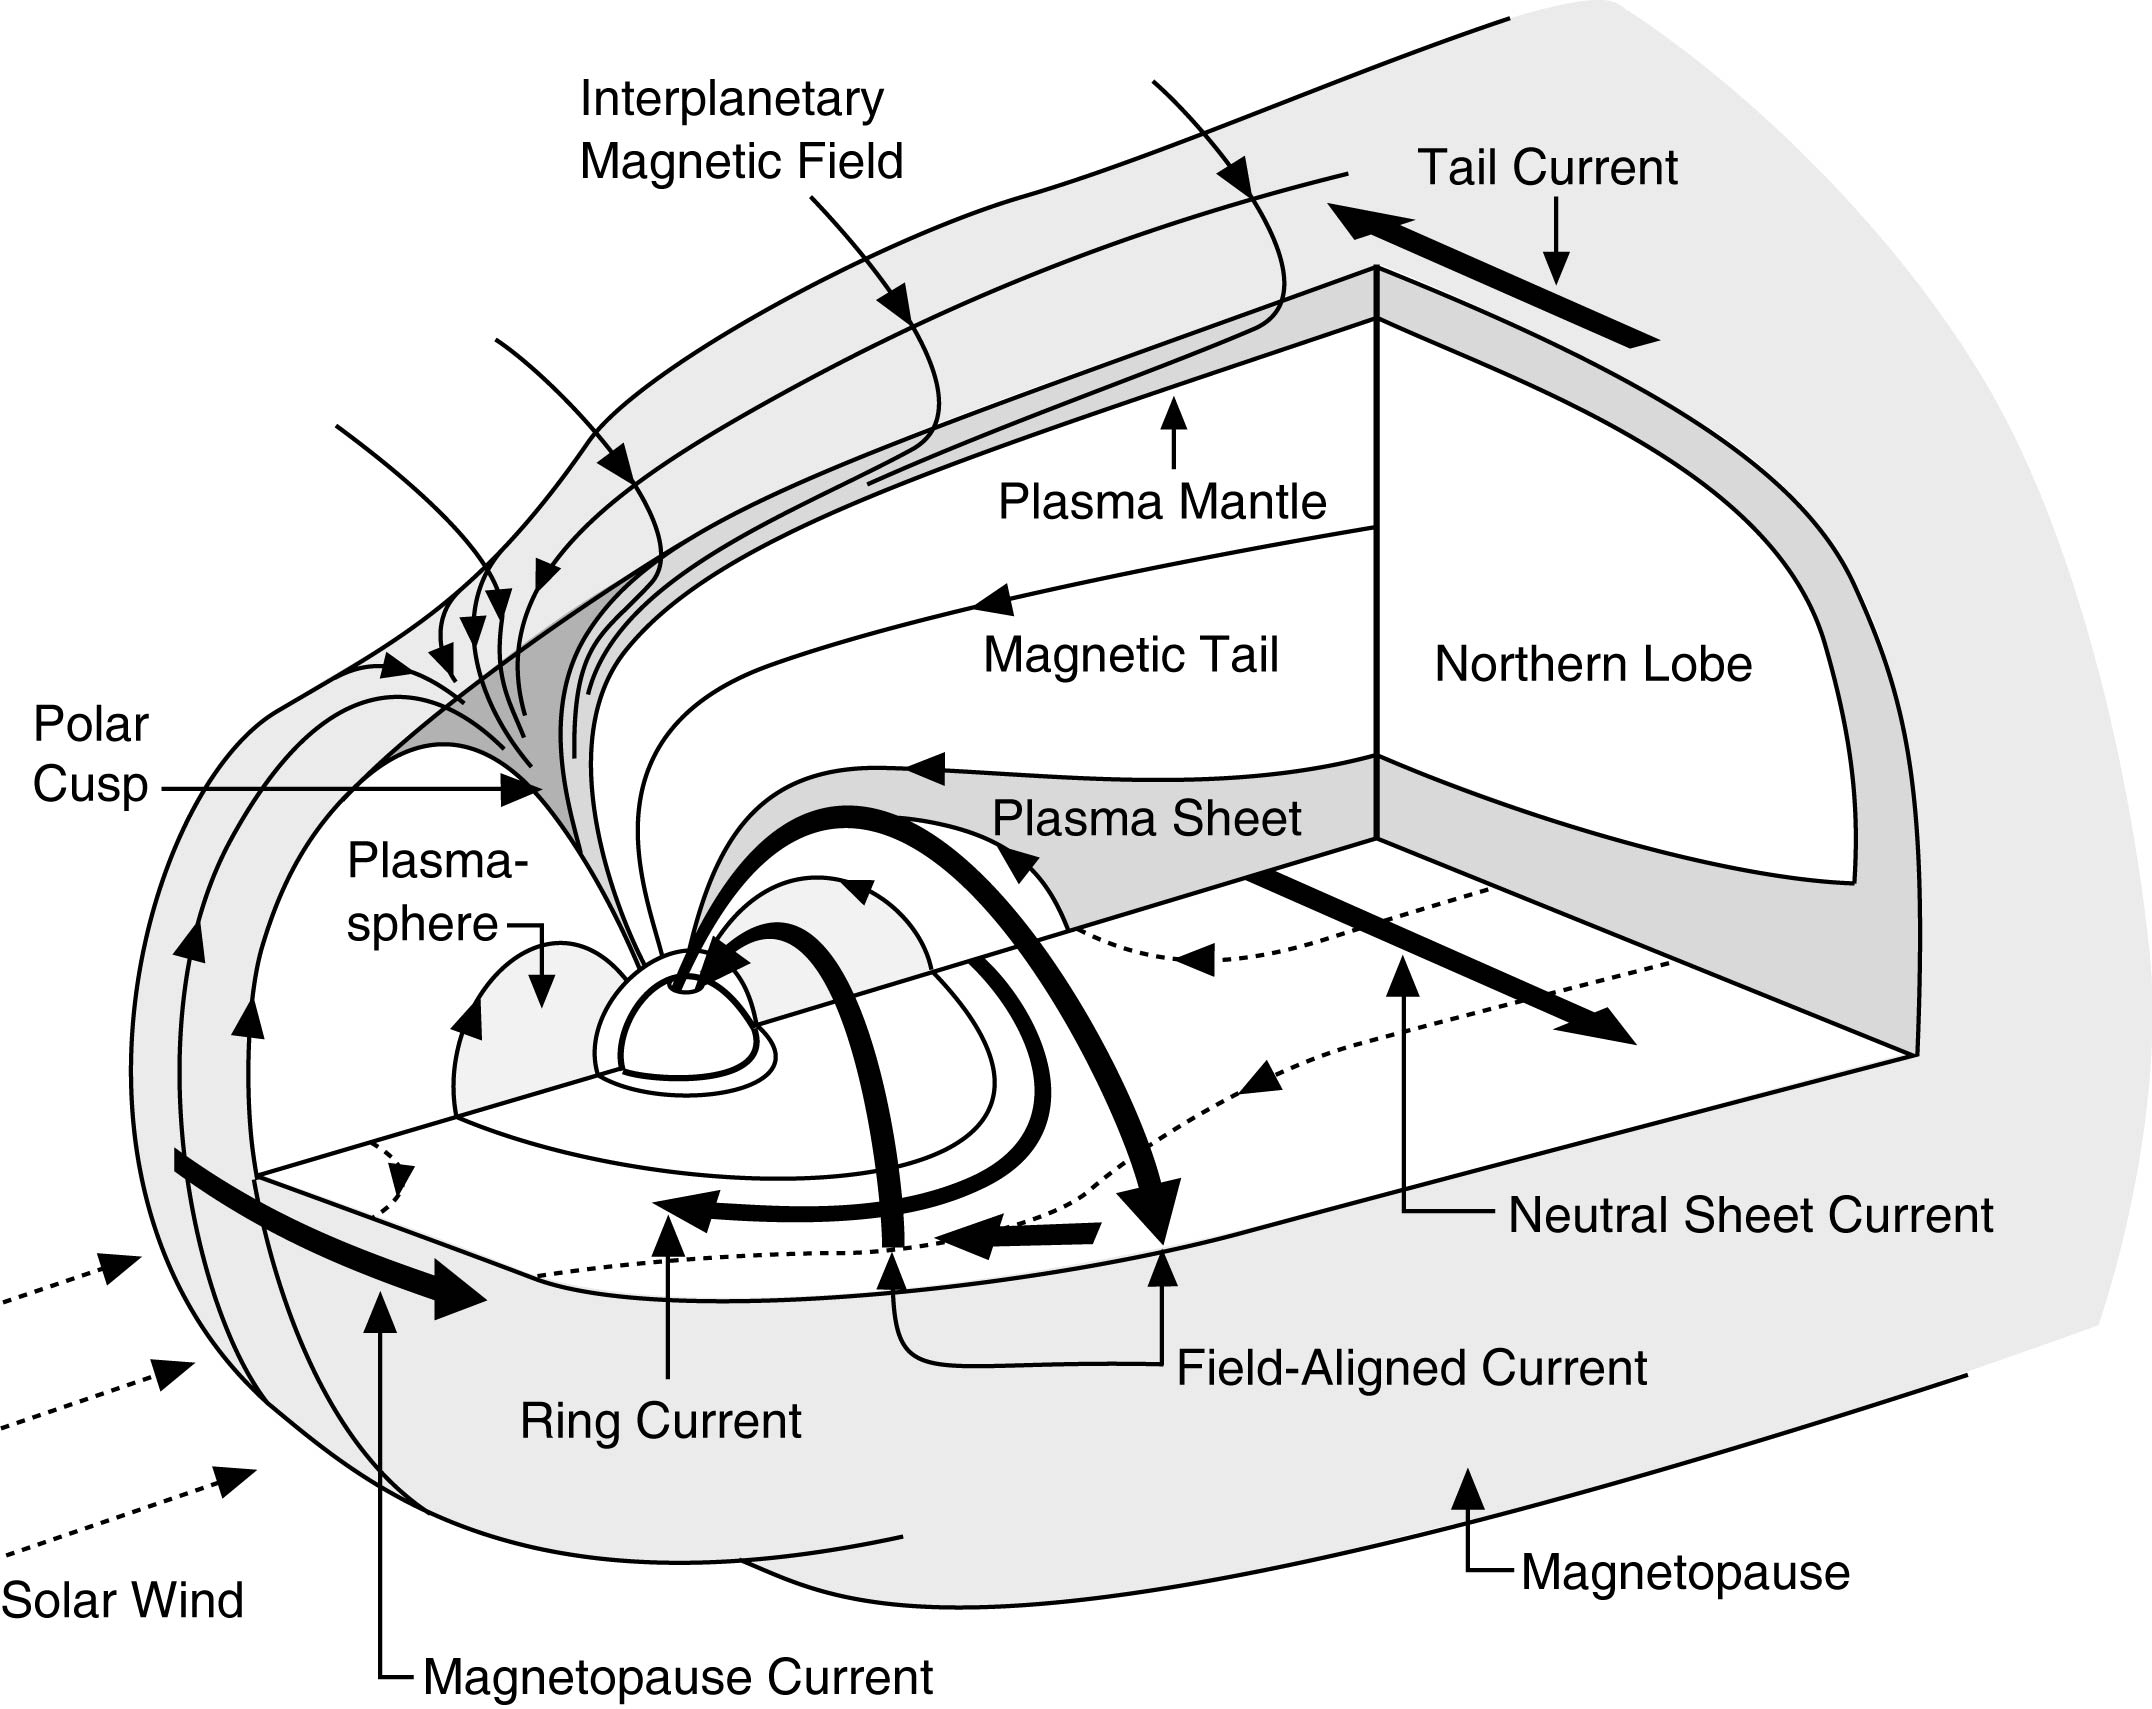
\includegraphics[width=0.8\textwidth]{intro/magnetospherediagram.jpg}
\caption[Diagram of Earth's magnetosphere.]{Diagram of the main features of Earth's magnetosphere from \citet{russell2016}, reproduced with permission.}
\label{intro:fig:magnetosphere}
\end{figure}

It can be seen that the magnetosphere is approximately dipolar in configuration on the dayside (i.e. the side facing the Sun), with a more extended `tail' on the nightside (i.e. the anti-sunward side), where the magnetic field lines stretch radially outwards and become approximately parallel to the solar wind direction. This tail can extend to tens or hundreds of planetary radii downstream of the planet; Jupiter's magnetotail has even been observed to extend as far as the orbit of Saturn, corresponding to several thousand Jovian radii downstream \citep{scarf1981}. Figure~\ref{intro:fig:magnetosphere} shows an azimuthal ring current system which orbits the planet near the equatorial plane; the direction is determined by the direction of the curvature and gradient drift velocities for positively charged particles in Earth's magnetic field, as described in Section~\ref{intro:sec:singleparticle} for the oppositely-oriented Saturn case. On the nightside this ring current extends into a current sheet, which separates the oppositely directed magnetic field lines in the northern and southern `lobes' of the magnetosphere. Currents also flow on the magnetopause and magnetotail surfaces as shown, separating the magnetic fields of the magnetosphere and the solar wind IMF. At the polar cusps, the magnetosphere is said to be `open' to the solar wind, as in these regions the internal planetary dipole magnetic field structure allows solar wind particles to access the magnetosphere. This is in contrast to the `closed' regions of the magnetosphere, where it is difficult for solar wind particles to penetrate.

\subsection{Comparative Magnetospheres}\label{intro:sec:comparativemagnetospheres}
A comparison of the magnetospheres of different planet systems is shown in Figure~\ref{intro:fig:magnetospherecomparison}. The most striking difference is in the overall size of the magnetospheres, and this is mainly due to the twin influences of the external solar wind conditions at each planet, and internal magnetic pressure associated with the planetary magnetic field. Table~\ref{intro:table:magnetospherecomparison} provides some typical parameters for the planets Earth, Jupiter and Saturn that help illustrate this. For example, the Jovian planetary dipole magnetic moment is some 20,000 times greater than that of Earth, with correspondingly higher magnetic field strength. This therefore means a much greater magnetic pressure inside Jupiter's magnetosphere. In addition, he solar wind dynamic pressure $D_\mathrm{P}$ is defined by 
\begin{equation}\label{intro:eq:dp}
D_\mathrm{P} = \rho_\mathrm{m}u_\mathrm{SW}^2
\end{equation}
where $\rho_\mathrm{m}$ is the mass density of the solar wind and $u_\mathrm{SW}$ is the velocity. As discussed in Section~\ref{intro:sec:solarwind}, $\rho_\mathrm{m}$ falls approximately as $r^{-2}$ while $u_\mathrm{SW}$ remains approximately constant, and so the external solar wind dynamic pressure is much lower for the planets in the outer solar system, falling as $r^{-2}$ .
\begin{figure}
\centering
\noindent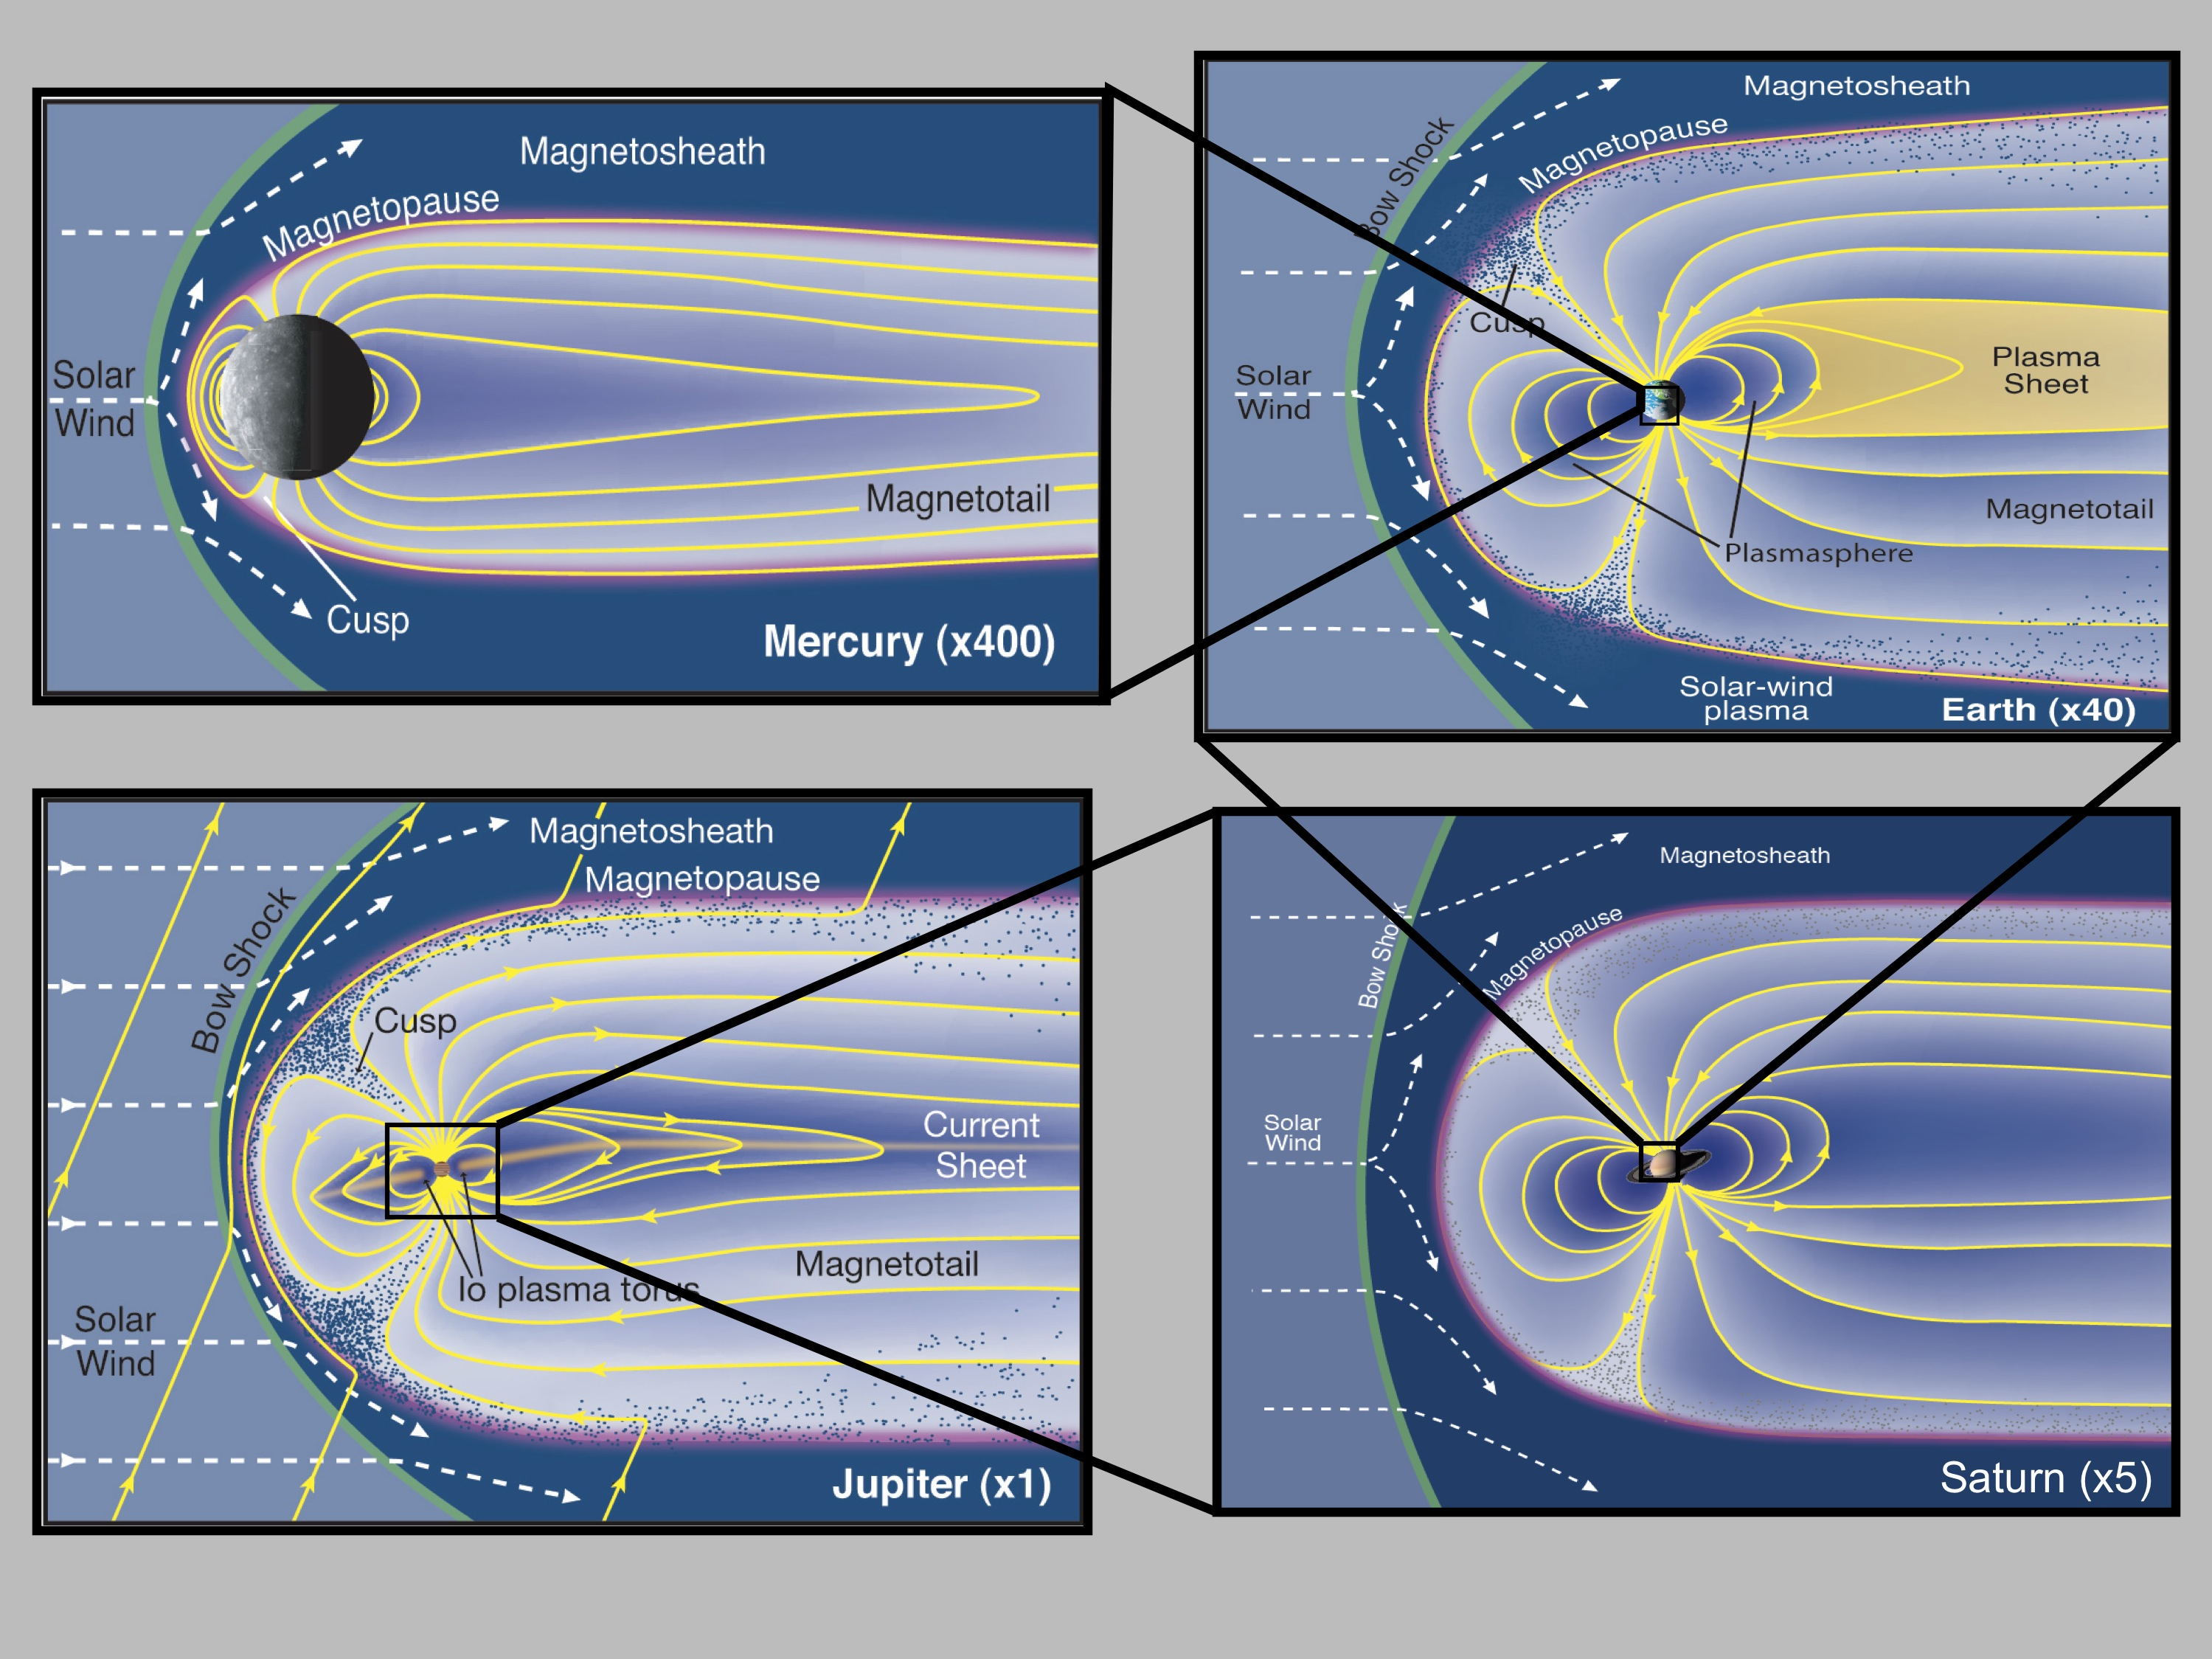
\includegraphics[width=1\textwidth]{intro/magnetospherecomparison.jpg}
\caption[Diagram of Mercury, Earth, Jupiter and Saturn magnetospheres.]{Diagram comparing the relative sizes and shapes of the magnetospheres of Mercury, Earth, Jupiter and Saturn, from Fran Bagenal and Steve Bartlett at LASP.}
\label{intro:fig:magnetospherecomparison}
\end{figure}
\begin{table}
\caption[Comparison of typical magnetospheric parameters for Earth, Jupiter and Saturn.]{Comparison of typical magnetospheric parameters for Earth, Jupiter and Saturn, adapted from \citet{bagenal2014} and references therein.$\SI{1}{M_\mathrm{EARTH}} = \SI{7.9D15}{\tesla \m^3}.$}\label{intro:table:magnetospherecomparison}
\centering
\begin{tabular}{l c c c}
\hline
 																															& Earth						& Jupiter			& Saturn  \\
\hline
Planet radius $R_\mathrm{P}$ ($\si{km}$)															& $\num{6371}$					&	$\num{71492}$			&	$\num{60268}$ \\
Distance from Sun ($\si{AU}$)																			&	1							&	5.2				& 9.6		\\
Solar wind number density ($\si{cm^{-3}}$)														& 7							&	0.2				&	0.07		\\
Spin period ($\si{hr}$)																						&	24						& 	9.9				&10.6		\\
Magnetic moment ($\si{M_\mathrm{EARTH}}$)													&	1							&	20,000			&	600		\\
Equatorial surface magnetic field ($\si{nT}$)														&	$\num{30600}$					&	$\num{430000}$		&	$\num{21400}	$\\
Dipole stand-off distance $R_\mathrm{CF}$	($\si{R_\mathrm{P}}$) 				&	$\SI{10}{R_\mathrm{E}}$ & $\SI{46}{R_\mathrm{J}}$ & $\SI{20}{R_\mathrm{S}}$ \\
Observed stand-off distance $R_\mathrm{MP}$ ($\si{R_\mathrm{P}}$)			&	$8-\SI{12}{R_\mathrm{E}}$ & $63-\SI{92}{R_\mathrm{J}}$ & $22-\SI{27}{R_\mathrm{S}}$ \\
\hline
\end{tabular}
\end{table}

This pressure-balance relationship is reflected in the `dipole stand-off distance' $R_\mathrm{CF}$ for each planet given in Table~\ref{intro:table:magnetospherecomparison}, where CF stands for Chapman-Ferraro as it was derived by \citet{chapman1930}. This distance is a theoretical location of the magnetopause, measured from the planet centre to the sub-solar point on the magnetopause surface, which would be expected if the external solar wind dynamic pressure was balanced exactly by the magnetic pressure associated only with an internal \textit{dipole} magnetic field. We can see that it is much greater for Jupiter and Saturn than for Earth, as expected from the pressure-balance explanation just given.

However at Saturn and Jupiter in particular, the observed magnetopause stand-off distances are significantly larger even than the Chapman-Ferraro estimates. This is mainly due to the significant internal plasma sources at each planet. At Saturn, the icy moon Enceladus orbits at a distance of $\SI{3.95}{R_\mathrm{S}}$, (where $\si{R_S}$ is the radius of Saturn, $\SI{60268}{km}$) and ejects water group molecules into the magnetosphere at around \SI{150}{kg s^{-1}} \citep{tokar2006,dougherty2006}. At Jupiter, the volcanic moon Io orbits at $\SI{5.9}{R_\mathrm{J}}$ (where $\si{R_J}$ is the radius of Jupiter, $\SI{71492}{km}$) and ejects sulphur dioxide into the magnetosphere at around \SI{1000}{kg s^{-1}}~\citep{bagenal2011}. At each planet, this material is partially ionised, forming a torus of plasma around each planet. The plasma pressure associated with this population adds to the internal magnetic pressure, inflating the magnetosphere beyond a dipolar internal field model. This is discussed in more detail in Section~\ref{intro:sec:pbalance}. In contrast at Earth, the Moon does not contribute a significant plasma population, and also mainly orbits the planet beyond the magnetosphere boundary, and so does not have the same influence on Earth's magnetosphere  \citep[e.g.][]{schneider1967}.

For Jupiter and Saturn, these internal plasma populations not only influence the overall size of the magnetosphere but also the internal structure of the magnetic field. This is due to the rapid rotation rates of the two planets, shown by the short spin periods in Table~\ref{intro:table:magnetospherecomparison}. Due to the aforementioned frozen-in field theorem, the magnetospheric plasma is azimuthally accelerated towards co-rotation with the rapidly rotating magnetic field of the magnetosphere. The centrifugal force associated with this confines the plasma towards the rotational equator, creating a thick plasma sheet. In order to balance this centrifugal force, the magnetic field is distorted around the plasma sheet from a dipolar magnetic field into a disc-like \textit{magnetodisc} structure, with a strong associated magnetic curvature force. This is characterised by field lines that are stretched radially outwards near the equatorial plane in outer magnetosphere, as can be seen particularly for Jupiter in Figure~\ref{intro:fig:magnetospherecomparison}, and is supported by the azimuthal ring current. The intensity of the ring current is enhanced by a population of hotter, more variable plasma that originates in the outer magnetosphere at both Saturn~\citep[e.g.][]{sergis2010} and Jupiter~\citep[e.g.][]{mauk2004}, with observed plasma $\beta$ of the order $2-5$ and ${\sim}100$ for these populations respectively. The magnetic field strength of this disk-like magnetic field structure in general varies more slowly with radial distance than a dipolar magnetic field, and thus also influences pressure balance at the magnetopause. This is investigated for both Saturn and Jupiter in Chapter~\ref{chap:compress}. 

\subsection{Magnetospheric Dynamics}\label{intro:sec:dynamics}
The simplest dynamical process that a magnetosphere undergoes is compression and expansion under varying solar wind conditions. For example, as the local solar wind dynamic pressure increases, due to an increase in velocity or number density by some process as described in Section~\ref{intro:sec:solarwind}, the magnetosphere is compressed. This compression causes the internal magnetic field pressure to increase, until it balances the enhanced external solar wind dynamic pressure and a new equilibrium magnetopause location is reached. If the solar wind pressure decreases, the magnetosphere then inflates. The magnetopause is therefore in constant motion, with a velocity or order $\SI{10}{kms^{-1}}$ at Earth \citep{berchem1982} and $\SI{100}{kms^{-1}}$ at Saturn \citep{masters2011}. The exact response of the magnetosphere to varying $D_\mathrm{P}$ varies significantly between planets due to the different internal structures. For Saturn in particular, the distance that the magnetopause location shifts for a given change in $D_\mathrm{P}$, and how this varies with different internal and external conditions, is the subject of the study in Chapter~\ref{chap:compress}, and is discussed in detail there.

However even under approximately constant solar wind conditions, a magnetosphere is not a static object. At the `solar-wind driven' magnetospheres Earth and Mercury, the dominant large-scale dynamic process is known as the \textit{Dungey Cycle}, after \citet{dungey1961}. A diagram of this process is shown in Figure~\ref{intro:fig:dungeycycle}. For an IMF oriented anti-parallel to the planetary magnetic field, conditions are favourable for reconnection of the two magnetic fields at the dayside magnetopause, as the magnetic field varies on small spatial scales (as discussed in Section~\ref{intro:sec:frozenin}). The planetary magnetic field lines are then open to the solar wind at one end whilst still anchored to the planet at the other, and are thus convected by the solar wind flow downstream to the nightside. This leads to a build-up of magnetic flux on field lines in the magnetotail, which then reconnect across the tail current sheet. This causes plasma to return on closed field lines back towards the planet on the nightside. At Earth, this process is associated with the generation of aurora along the boundary between open and closed magnetic field lines, in the northern and southern polar atmospheres \citep[e.g.][]{milan2007}. As the energetic electrons in the plasma gyrate around the polar magnetic field lines towards the planet, they excite atoms in the atmosphere, which then decay back to a lower energy level and emit photons in the process, which are observed as aurora.

\begin{figure}
\centering
\noindent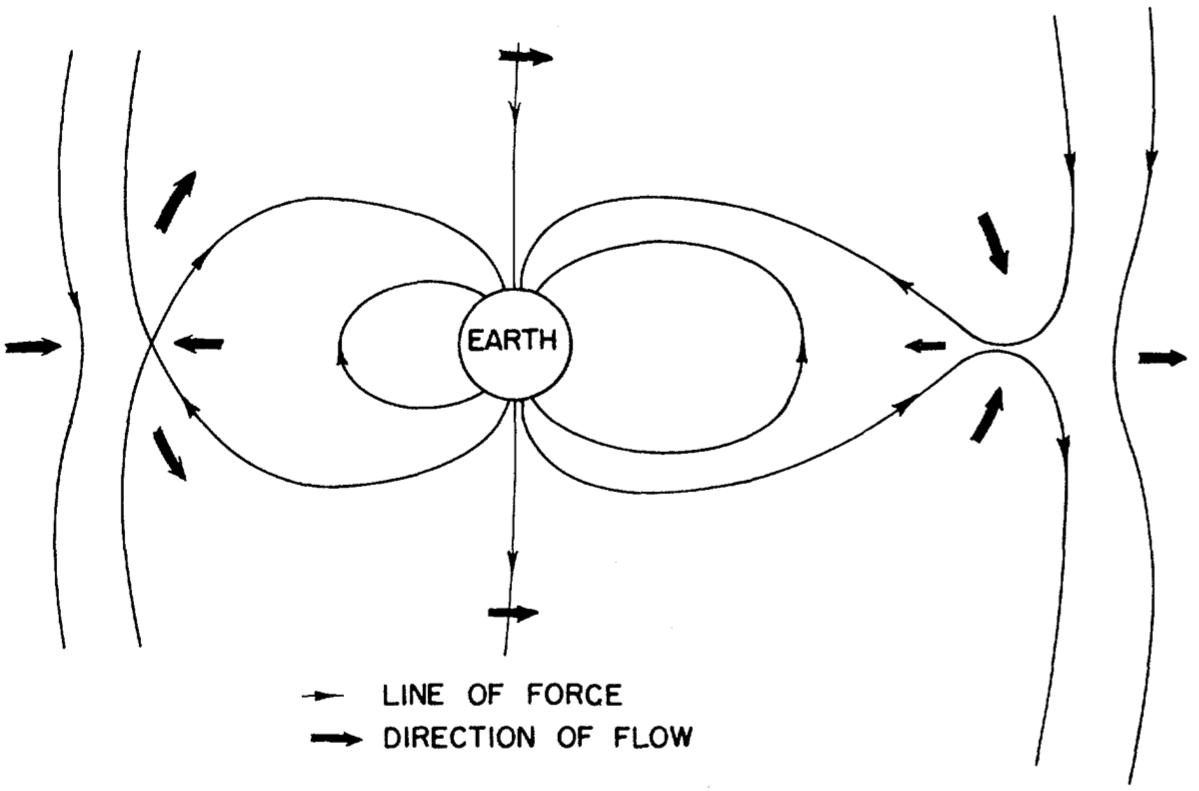
\includegraphics[width=0.8\textwidth]{intro/dungeycycle.png}
\caption[Diagram of the Dungey cycle.]{Diagram showing the Dungey Cycle process at Earth, from \citet{dungey1961}. Thin black `lines of force' are magnetic field lines. The solar wind flows from left to right.}
\label{intro:fig:dungeycycle}
\end{figure}

At Jupiter and Saturn, the dominant dynamical process is driven by the rapid planetary rotation, and thus we say they are `rotationally driven' magnetospheres. This process is known as the Vasyliunas cycle, after \citet{vasyliunas1983}, and a diagram depicting it is shown in Figure~\ref{intro:fig:vasyliunascycle}. As discussed in the previous section, these rapidly rotating magnetospheres have significant internal plasma populations, which are accelerated to near-corotation with the rotating planetary magnetic field. The centrifugal interchange instability causes this plasma to be transported radially outwards, such that inner cold, dense flux tubes are exchanged with outer hot, tenuous flux tubes \citep{southwood1989}, and the magnetic field is stretched out as shown in region 1 of Figure~\ref{intro:fig:vasyliunascycle}. As the flux tubes rotate around to the nightside, they are no longer as confined by the magnetopause boundary and so expand down the tail, and the magnetic field becomes increasingly more stretched (region 2) until reconnection occurs across the tail (region 3). This generates the release of a `plasmoid' down the tail, and the newly empty flux tube is then convected back around the planet on the dawn side. 

This cycle is dominant over the Dungey cycle for the outer giant planets due to the combined effects of the much faster rotation rates, and overall larger magnetospheric sizes, which means a much longer period of time for a magnetic field line to be convected across the polar cap from dayside to nightside \citep{forsyth2010}. However at Saturn in particular, it still uncertain how much of a role the Dungey cycle has to play \citep[e.g.][]{cowley2005}.

\begin{figure}
\centering
\noindent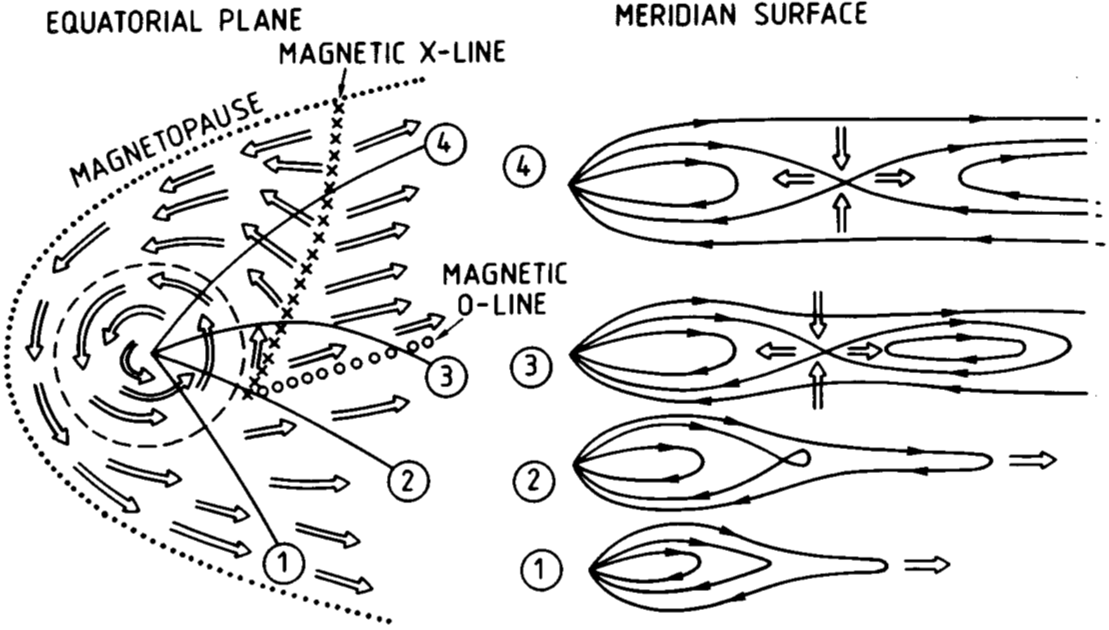
\includegraphics[width=0.9\textwidth]{intro/vasyliunascycle.png}
\caption[Diagram of the Vasyliunas cycle.]{Diagram showing the Vasyliunas cycle of plasma transport, from \citet{vasyliunas1983}. The dotted line shows the magnetopause boundary, the dashed line shows the region where plasma perfectly corotates with the magnetic field, and empty arrows show the plasma flow direction.}
\label{intro:fig:vasyliunascycle}
\end{figure}

In addition to these main modes of plasma transport in planetary magnetospheres, there are also numerous small-scale dynamical processes, such as Kelvin-Helmholtz vortices on the magnetopause surface; however these vary significantly between planets and are not relevant to the work of this thesis, and so we do not cover them explicitly here.

\section{Saturn and its Magnetosphere}\label{intro:sec:saturn}
%\subsection{Configuration of Saturn's Magnetosphere}
Saturn orbits the Sun once every ${\sim}29$ years, on an elliptical orbit at an average distance of \SI{9.6}{AU}. Saturn is approximately 10 times the size of Earth (by radius), and around 100 times as massive, meaning its density is around 1/10 Earth's. This is because Saturn is a `gas giant' planet, composed mainly of molecular hydrogen and helium, with a small rocky core. Between the core and the outer layers, the hydrogen is compressed to such high pressures and temperatures that it becomes `metallic', flowing and conducting electricity and generating the dynamo of Saturn's planetary magnetic field.

The internal planetary magnetic field is approximately dipolar, though with smaller higher order moments, and is offset northwards from the planetary equator by ${\sim}\SI{0.05}{R_S}$ \citep{dougherty2018}. Arguably the most interesting aspect of Saturn's internal magnetic field is that the dipole axis is extremely closely aligned with the planet spin axis, with the same study by \citet{dougherty2018} finding an upper limit of $\SI{0.01}{\degree}$ difference between them. This is seemingly in contradiction with Cowling's Theorem, which states that an active dynamo cannot maintain a perfectly axisymmetric magnetic field \citep{cowling1933}. This extreme axisymmetry also means it is near impossible to determine the rotation rate of the planet's deep interior; however, a range of periodic phenomena are observed at Saturn at periods assumed \textit{close} to the true planetary rotation rate, as discussed in detail in Section~\ref{intro:sec:periodicities}.

From Table~\ref{intro:table:magnetospherecomparison} and the associated discussion, we have seen that in many ways Saturn's magnetosphere is an intermediate between Earth and Jupiter. It is therefore a particularly interesting system to study, and can be used to learn more about magnetospheric physics in a global context. Saturn's magnetosphere was first investigated \textit{in situ} with single flybys by the outer solar system space missions \textit{Pioneer} (1979), \textit{Voyager I} (1980) and \textit{Voyager II} (1981). These observations did not reveal a significant magnetodisc magnetic field structure on Saturn's dayside (as was known to exist at Jupiter), although did provide some evidence for a thin current sheet on the dawn flank \citep{smith1980}. However with the arrival of the \textit{Cassini} space mission into orbit around Saturn in 2004, and its continued observation of the system until late 2017, our scientific understanding of Saturn's magnetosphere has been revolutionised. (The \textit{Cassini} space mission is discussed in detail in Chapter~\ref{chap:cassini}.)

We now know that in the outer magnetosphere, a non-negligible magnetodisc magnetic field structure exists at all local times beyond a radial distance of ${\sim}\SI{15}{R_S}$, due to the reasoning discussed in Section~\ref{intro:sec:comparativemagnetospheres}. However particularly on the dayside, it was found that a significant magnetodisc structure only forms under low solar wind dynamic pressure, where the subsolar magnetopause stand-off distance becomes greater than $\SI{23}{R_S}$, and that when it is more extremely compressed than this, the magnetic field remains approximately dipolar~\citep{arridge2008}. It is interesting that this value falls between the two modes of the bimodal distribution in magnetopause stand-off distances observed by \citet{pilkington2015}, of $\SI{20.7}{R_S}$ and $\SI{27.1}{R_S}$. This behaviour is broadly due to overall force balance in Saturn's magnetosphere; for a more expanded system, the magnetic field strength is weaker in the outer magnetosphere, and so a larger magnetic tension force is needed to balance the centrifugal and plasma pressure gradient forces acting radially outwards on the plasma. In Chapter~\ref{chap:compress} of this thesis, we present results that show the compressibility of the magnetosphere also changes behaviour at around this value of stand-off distance, at ${\sim}\SI{25}{R_S}$. 

The formation of a magnetodisc structure at Saturn is also influenced by the variable hot plasma population observed by \citet{sergis2010} and others, as discussed in Section~\ref{intro:sec:comparativemagnetospheres}, through an enhancement of the equatorial ring current intensity. By consideration of Amp\`ere's law, it can be understood that the magnetic field associated with an azimuthal current flowing in the direction of corotation decreases Saturn's planetary magnetic field in the inner magnetosphere, and increases it in the outer magnetosphere. This corresponds to a magnetodisc magnetic field structure. Many studies have attempted to characterise the thickness and radial extent of this equatorial ring current, using a combination of \textit{Cassini} data, and models such as that of \citet{connerney1981b, connerney1983}, which assumes an azimuthally symmetric current loop of uniform thickness. The nature of the ring current has been observed to vary significantly over time, with location, and with system size \citep[e.g.][]{bunce2007}, with a variable thickness of average ${\sim}\SI{3}{R_S}$ and significant radial extent, from around $\SI{7}{R_S}$ out to around $\SI{18}{R_S}$, at times reaching the magnetopause boundary on the dayside \citep[e.g.][]{kellett2009,sergis2009}. However due to incomplete coverage particularly across local time for most of the \textit{Cassini} mission, it was not until near the end of the mission that the local time asymmetry of the ring current was demonstrated by \citet{sergis2017}. Indeed, the local time variation in the large scale structure of Saturn's magnetosphere is still not fully understood, and is studied in this thesis in Chapter~\ref{chap:LTsectors} using a flexible model of the ring current adapted from \citet{achilleos2010a}.

\subsection{Planetary Period Periodicities}\label{intro:sec:periodicities}
%The equatorial current sheet is just one part of Saturn's magnetosphere that displays periodic dynamical behaviour, at a rate close to the planetary rotation rate. At Jupiter, the dipole axis is tilted relative to the rotation axis by $\SI{9.4}{\degree}$. The current sheet lies in the \textit{magnetic} equatorial plane, and so for a stationary observer, the current sheet appears to `flap' above and below the rotational equator once per planetary rotation. Similar behaviour is observed at Saturn, despite the aforementioned alignment oft the dipole and rotation axes, and hence must be caused by a more complicated process.
%Dynamic current sheet. A summary of periodicities, the history, the different values, when and where they were discovered and what they might mean.
Another key aspect of Saturn's magnetosphere that is still not fully understood, is the nature of the observed periodic variations in field and particle properties. These variations, summarised in \citet{carbary2013}, have periods ranging from around 10.6-10.8 hours, assumed close to the true planetary rotation rate. Magnetospheric periodicities include the location of the auroral oval \citep{provan2009b}, and the magnetopause boundary \citep{clarke2010}; the magnetic field strength and direction \citep{espinosa2000, andrews2008}; electron densities \citep{morooka2009}; ion distributions \citep{burch2009}; and energetic neutral atoms \citep{paranicas2005}. These observations are especially interesting due to the aforementioned axisymmetry of Saturn's magnetic field, which means they cannot be adequately explained by a geometric tilt of the magnetic field. In addition, some of the observed periods vary relatively quickly, by up to $1\%$ over the course of a year, and thus cannot be associated with changes to the planet's deep interior. This complex behaviour is apparently unique to Saturn, and has made it impossible to measure Saturn's true core rotation rate.

Initially, periodicities in radio observations of Saturn's auroral regions from the \textit{Voyager} spacecraft suggested a planetary rotation period of $\SI{10.657}{\hour}$ \citep{desch1981}. This radio emission is known as Saturn Kilometric Radiation, or SKR. However observations from the \textit{Ulysses} \citep{lecacheux1997} and later \textit{Cassini} \citep{gurnett2005} missions revealed that the SKR period was actually drifting over time, and thus could not be associated with the core rotation rate. A reanalysis of magnetometer data from the \textit{Voyager} and \textit{Pioneer} missions then showed a similar periodic behaviour in the magnetic field. This led to the development of a `camshaft' model, where a rotating equatorial magnetic anomaly that is fixed in longitude triggers radial waves that cause the observed perturbations \citep{espinosa2003b}. To further complicate the picture, two distinct periods were then discovered in the SKR signal by \textit{Cassini}, associated separately with the Northern and Southern hemispheres \citep{gurnett2009}. This phenomenon was then also observed in more recent \textit{Cassini} magnetic field observations \citep[e.g.][]{andrews2010,provan2012}. In these and other studies, such as \citet{hunt2014}, a picture has now been developed of how these hemispheric magnetic perturbations are generated, by two large-scale field-aligned current systems that rotate at slightly different rates in each hemisphere. The magnetic field associated with each current system is dominant in the respective hemisphere, and can be approximated in the outer magnetosphere by a rotating, transverse oriented dipole. However the true magnetic field perturbation is much more complex, and is currently an area of active research, with some final \textit{Cassini} results still to be fully analysed. The physical origins of these current systems are also still not fully understood, but are thought to be associated with twin atmospheric vortices flowing in the polar upper atmosphere/ionosphere in each hemisphere \citep{jiaandkivelson2012, southwood2014, smith2016}. 

In the equatorial plane, these magnetic field perturbations have the effect of making Saturn's current sheet appear to`flap' above and below the rotational equator once per planetary rotation \citep[e.g.][]{arridge2011}. Similar behaviour is also observed at Jupiter. However Jupiter the dipole axis is tilted \SI{9.4}{\degree} relative to its rotation axis, which means that relative to the rotational equator, the current sheet behaves approximately as a rotating, tilted disc, and so this behaviour is expected. In addition, at Saturn, these periodic magnetic field perturbations also have the effect of periodically thickening and thinning the current sheet at different longitudes \citep{provan2012}, associated with a large scale compression and expansion of the magnetosphere in a given region, known as `breathing' \citep{ramer2016}. Both the `flapping' and `breathing' behaviours are controlled by the relative phases of the northern and southern magnetic perturbations, noting that their independent rotation rates means the phase relationship between them changes over time. This complicated dynamical behaviour is the focus of much current research, and is the subject of the study in Chapter~\ref{chap:equinox}.

\subsection{Pressure Balance at the Magnetopause}\label{intro:sec:pbalance}
As previously mentioned, the magnetopause boundary can be approximated as the location where the effective pressure of the solar wind exerted on the magnetosphere is exactly balanced by the sum of the internal magnetospheric particle and field pressures. 

Before impacting on the magnetopause, the solar wind flow is first decelerated via the bow shock, and is deflected around the magnetosphere obstacle. This acts to reduce the dynamic pressure incident on the magnetopause surface, and must be accounted for when considering pressure balance. \citet{petrinec1997} used Bernoulli's equation in combination with the Rankine-Hugoniot jump conditions across the bow shock, assuming adiabatic flow of the solar wind, to show that the relation
\begin{equation}\label{intro:eq:pbalance1}
\frac{B_{\mathrm{MS}}^2}{2\mu_0} + P_{\mathrm{MS}} = kD_\mathrm{P}\cos^2\psi + P_0\sin^2\psi
\end{equation}
provides an approximation that is valid across the magnetopause surface, not just at the nose. For clarity the subscript {\sc{MS}} denotes magnetospheric properties, such that the terms on the left hand side of equation \ref{intro:eq:pbalance1} are the magnetospheric magnetic and plasma pressures respectively. $\psi$ is the flaring angle measured between the upstream flow velocity vector and the normal to the magnetopause surface, such that $\psi=0$ at the nose and generally increases as you move anti-sunward along the magnetopause surface. The first term on the right hand side is associated with the solar wind dynamic pressure, where $k$ is a positive constant $\leq1$ to account for the aforementioned diversion of flow, and the $\cos^2\psi$ factor accounts for the reduction in the normal component of dynamic pressure on the flanks and tail of the magnetosphere. The second term on the right hand side is composed of a `static' pressure $P_0$ associated with the thermal pressure of the solar wind, and a $\sin^2\psi$ factor to ensure a real (i.e. not imaginary) flow velocity in the subsolar region \citep[see][]{petrinec1997}.

In order to improve agreement with the results of MHD simulations from \citet{hansen2005}, and to improve the consistency of $D_\mathrm{P}$ estimates, \citet{kanani2010} proposed a modification to this relation such that $P_0$ is dependent on $D_\mathrm{P}$. The relationship then becomes

\begin{equation}\label{intro:eq:pbalance2}
\frac{B_\mathrm{MS}^2}{2\mu_0} + P_\mathrm{MS} = \left[k\cos^2(\psi) + \frac{k_\mathrm{B}T_\mathrm{SW}}{1.16m_\mathrm{p}u_\mathrm{SW}^2}\sin^2(\psi)\right] D_\mathrm{P}
\end{equation}

where $k_\mathrm{B}$ is the Boltzmann constant, $m_\mathrm{p}$ is the mass of a proton, and $T_\mathrm{SW}$ and $u_\mathrm{SW}$ are the solar wind temperature and velocity respectively. The value of $k$ depends on the ratio of specific heats $\gamma$ in the solar wind, and the upstream sonic Mach number $M$. For high (${\gtrsim}8$) Mach number flow with $\gamma = 5/3$, $k = 0.881$ \citep{spreiter1966}, which is a valid assumption for the solar wind at Saturn's orbit \cite[e.g.][]{slavin1985,achilleos2006}.

This relationship allows an approximation of the solar wind dynamic pressure to be made, when only internal information about the state of the magnetosphere is known. 
Thus this relation is often used in studies that attempt to model the shape and size of the magnetopause boundary in response to changing $D_\mathrm{P}$, using only \textit{in situ} \textit{Cassini} data about the magnetic and plasma pressure inside the magnetosphere. These studies are discussed in more detail in Chapter~\ref{chap:compress}.

\section{The UCL/AGA Force-Balance Model of Saturn's Magnetodisc}\label{intro:sec:forcebalancemodel}
Throughout this thesis we will employ the University College London/Achilleos-Guio-Arridge (UCL/AGA) magnetodisc model from \citet{achilleos2010a,achilleos2010b}, with appropriate modifications as described in each chapter. This model is based on a magnetic field and plasma model originally constructed for the Jovian magnetodisc by \citet{caudal1986}, and adapted for the Saturn system. More information can be found in \citet{achilleos2010a, achilleos2010b}. The model is axisymmetric about the planetary dipole/rotation axis, which are assumed to be parallel. This parallel assumption is appropriate for Saturn in particular, as the rotation and dipole axes are aligned to within \SI{0.01}{\degree} \citep{dougherty2018}. This axisymmetric assumption is appropriate as an approximation of the large-scale structure of the magnetic field, as shown by \citet{hunt2014}, who compared the gradients of currents in radial, azimuthal and meridional directions and found the azimuthal gradients could be neglected. It is constructed based on the assumption of force balance in the rotating plasma of the magnetosphere between the Lorentz body force (including magnetic pressure and tension forces), pressure gradient force and centrifugal force, such that 
\begin{equation}\label{intro:eq:forcebalance}
\boldsymbol{J} \times \boldsymbol{B} = \nabla P - nm_i\omega^2\rho\boldsymbol{\hat{\rho}}
\end{equation}
where $\rho$ is cylindrical radial distance from the axis, with $\boldsymbol{\hat{\rho}}$ its unit vector. The plasma properties are isotropic pressure $P$, temperature $T$, ion number density $n$, mean ion mass $m_i$ and angular velocity $\omega$. Note that this construction is equivalent to equation~\ref{intro:eq:momentum}, the MHD momentum equation, with simplifying assumptions as described in that section, assuming force balance such that the acceleration of the plasma is zero, and including the centrifugal force on the plasma associated with the planetary rotation.

As a consequence of Maxwell's equation~\ref{intro:eq:nomonopoles}, any magnetic field can be presented in terms of two Euler potentials $\alpha$ and $\beta$, such that 
\begin{equation}
\boldsymbol{B} = \nabla \alpha \times \nabla \beta.
\end{equation}
(Note this has no relation to the plasma $\beta$, ratio of plasma to magnetic pressure.) For an axisymmetric field with no azimuthal component, the forms of $\alpha$ and $\beta$ can be chosen such that the magnetic field configuration is fully defined by one Euler potential which we call $\alpha = \alpha(r,\mu)$, where $r$ is radial distance from the origin, and $\mu = \cos\theta$, the cosine of colatitude. Using this form of $\alpha$, \citet{caudal1986} demonstrated that equation~\ref{intro:eq:forcebalance} is equivalent to the partial differential equation
\begin{equation}\label{intro:eq:pde}
\frac{\partial^2\alpha}{\partial r^2} + \frac{1-\mu^2}{r^2} \frac{\partial^2\alpha}{\partial \mu^2} = -g(r,\mu,\alpha)
\end{equation}
where $g(r,\mu,\alpha)$ is a source function determined by the distribution of plasma and angular velocity in $r,\mu$ space. This equation can be solved semi-analytically using Jacobi polynomials as laid out in detail in \citet[Appendix]{achilleos2010a} to give surfaces of constant $\alpha$, corresponding to magnetic field lines, in $r, \mu$ space. The model solution also provides a prediction of the local plasma pressure, and the azimuthal current density components associated with each of the terms on the right hand side of equation \ref{intro:eq:forcebalance}. 

Since the source function is itself dependent on $\alpha$, equation \ref{intro:eq:pde} must be solved iteratively, starting from a pure dipole magnetic field and then successively perturbing it. At each iteration, a linear combination of the present solution $\alpha_i$ and the previous solution $\alpha_{i-1}$ is used as input for the next iteration calculation, such that
\begin{equation}\label{intro:eq:convergence}
\alpha_{i+1\mathrm{(input)}} = \gamma\alpha_i + (1-\gamma)\alpha_{i-1},
\end{equation}
where $\gamma<1$ controls the relative weighting between the previous and current solutions. This is a form of numerical relaxation. This $\alpha_{i+1(\mathrm{input})}$ is then used to calculate the source function in equation~\ref{intro:eq:pde} to solve for $\alpha_{i+1}$. In the original model construction, the two components were weighted equally ($\gamma=0.5$) and calculations continued until the maximum difference between successive iterations fell below a chosen `tolerance' $\delta = 0.5\%$, considered as convergence. In some of the work in this thesis we found that, for models with more extreme input parameters, it was necessary to weight the previous solution up to nine times more heavily than the present solution ($\gamma=0.1$), in order to achieve convergence. (Exactly what constitutes an `extreme parameter' will be discussed in future chapters.) In order to keep the ratio $\delta/\gamma$ constant at $10^{-2}$, and therefore consistent with the original model approach, this corresponds to using a more stringent stopping tolerance $\delta = 10^{-2}\times0.1 = 0.1\%$ in such cases.

The global plasma properties can then be inferred entirely from the calculated magnetic field structure, using appropriate boundary conditions, as follows. \citet{caudal1986} explained that as a consequence of equation~\ref{intro:eq:forcebalance}, with $T$ and $\omega$ constant along magnetic field lines (according to Liouville's theorem and Ferraro's isorotation theorem respectively), the plasma pressure P is determined by 
\begin{equation}\label{intro:eq:p}
P = P_{0}\exp\left(\frac{\rho^2-\rho_0^2}{2\ell^2}\right),
\end{equation}
where $\ell$ is the \textit{confinement scalelength} (in $\rho$)
\begin{equation}
\ell^2 = \frac{2k_BT}{m_i\omega^2}.
\end{equation}
The subscript 0 means the quantity evaluated at the equatorial crossing point of the magnetic field line. This represents the plasma being confined towards the rotational equatorial plane due to the centrifugal force exerted on it. The model assumes that the plasma is composed of a cold and hot population; for the hot plasma population, the thermal energy associated with the plasma is significantly greater than the centrifugal potential, and so $\ell^2$ tends to infinity, such that the hot plasma pressure is not confined to the equator but is constant along magnetic field lines, $P_\mathrm{H} = P_\mathrm{H0}$. This assumption is supported by observations such as \citet{krimigis2007}, who used data from the \textit{Cassini} MIMI instrument to show that the hot plasma population extends to high latitudes, particularly on the dayside, verifying that the plasma can effectively fill their flux tubes due to their high energies.  Hence, the full form of equation~\ref{intro:eq:p} is only necessary for calculating the cold plasma pressure.

The requisite boundary conditions for the model are, then, the equatorial radial profiles of plasma properties. These were obtained from studies using results mainly from \textit{Cassini} plasma instruments CAPS and MIMI/INCA, as summarized in \citet{achilleos2010a}, and updated in \citet{achilleos2010b}. For the cold plasma population, the profiles for $m_i$ and $T$ were obtained from \citet{wilson2008}, $\omega$ profiles from \citet{wilson2008} and \citet{kane2008}, and the flux tube content information from \citet{mcandrews2009}. For the studies described in Chapters \ref{chap:equinox} and \ref{chap:LTsectors} we updated some of these boundary conditions using more recent results from \citet{wilson2017}, as described in those chapters, with details in the Appendix~\ref{appendix:sec:wilsonfits}.

As the hot plasma pressure is assumed uniform along magnetic field lines, the plasma population may be completely characterised by a particular equatorial plasma pressure $P_\mathrm{H0}$ and flux tube volume $V$ per unit of magnetic flux, where
\begin{equation}\label{intro:eq:ftv}
V = \int_{0}^{s_{B}} ds/B,
\end{equation}
and $ds$ is an element of arc length along the magnetic field line. The integral limits represent measurement along a field line of total length $s_B$ between the southern and northern ionospheric footprints at $\SI{1}{R_S}$. The flux tube volume is therefore dependent on both the shape of magnetic field lines, via $ds$, and the strength of the field, via $B$. Studies using \textit{Cassini} MIMI data such as \citet{sergis2007} found that the equatorial pressure associated with the hot plasma population was highly variable with $\rho$ and over time, as described in Section~\ref{intro:sec:saturn}. In light of these observations, the original \citet{achilleos2010a} model simply parameterised the global hot plasma content by a single `hot plasma index' $K_\mathrm{H}$, where $ K_\mathrm{H}= P_\mathrm{H0}V$ is constant beyond $\SI{8}{R_S}$, and $P_\mathrm{H0}$ decreases linearly to 0 inside that distance. A similar parameterisation, though with different values of the constants, was made in \citet{caudal1986}, who argued that for the Jovian system, under the expected conditions of rapid radial diffusion, the hot plasma would be transported isothermally. In \citet{achilleos2010a} the authors used a value of $K_\mathrm{H} = \SI{2e6}{Pa m T^{-1}}$ to represent `typical' hot plasma content conditions at Saturn, although results presented in that study suggest $K_\mathrm{H}$ may vary in the range $10^5{\--}10^7~\si{Pa m T^{-1}}$. Parameterising the hot plasma content in this way provides the flexibility to very simply characterize the level of ring current activity in the model, and thus investigate the effect of the varying hot plasma content on magnetospheric structure, and magnetospheric compressibility. This is the basis of the study described in Chapter~\ref{chap:compress}. In Chapter~\ref{chap:LTsectors}, this hot plasma pressure boundary condition is updated to describe different local time sectors, using recent results from \citet{sergis2017}.

Finally, at every iteration, a small uniform southward-directed `shielding field' is added to the magnetic field, in order to approximately account for the magnetic field associated with the magnetopause and magnetotail current sheets. Sketches of these current systems are included in the diagram in Figure~\ref{intro:fig:magnetosphere}, though note they are in the opposite sense for the Saturn system due to the opposite orientation of Saturn's planetary dipole. In \citet{achilleos2010a} the magnitude of this field was chosen by calculating dayside equatorial averages of the empirical field models of \citet{alexeev2005} and \citet{alexeev2006}, and it varied with model magnetodisc radius $R_\mathrm{D}$ \citep[see][Figure 6]{achilleos2010a}. In particular the component of the shielding field associated with the magnetopause currents was based on a dipole approximation of the magnetospheric magnetic field. In Chapter~\ref{chap:equinox} we update this calculation for a more realistic magnetodisc magnetic field, and in Chapter~\ref{chap:LTsectors} we modify this calculation using local time sector averages of the models of \citet{alexeev2005} and \citet{alexeev2006}, to account for the increased significance of the tail current field compared to the magnetopause current field for nightside local time sectors.

\section[Open Questions about Saturn's Magnetosphere]{Open Questions about Saturn's Magnetosphere: Motivations and Summary of this Thesis}
As a community, we are still trying to understand the large-scale structure of Saturn's magnetosphere, and how it varies in response to internal and external influences. We know that the rapid planetary rotation rate, significant internal hot and cold plasma populations, and external solar wind conditions all play a role in determining the configuration of the magnetosphere – but which factor is dominant, and does this relationship change under different conditions and in different places?

The answers to these questions have consequences for other areas of magnetospheric physics at Saturn. In Sections~\ref{intro:sec:comparativemagnetospheres} and \ref{intro:sec:pbalance} we touched on the concept of magnetospheric compressibility, and how the size of the magnetosphere scales with varying solar wind dynamic pressure. From equation~\ref{intro:eq:pbalance2}, it can be seen that the relative magnitudes of the magnetic and plasma pressures just inside the magnetopause are important in determining this pressure balance, and hence the system size. Therefore an investigation of the magnetospheric compressibility, and how it varies under different conditions, can reveal information about overall pressure balance within the magnetosphere. In Chapter~\ref{chap:compress} we investigate this compressibility using the \citet{achilleos2010a} magnetodisc model calculated at different system sizes. This approach complements previous observational studies based on \textit{Cassini} data, and also provides an opportunity to explicitly investigate the influence of the variable hot plasma population on the compressibility behaviour. We also use our results to make a direct comparison with the compressibility of Jupiter's magnetosphere, to test our expectations that Saturn behaves as an intermediate between Earth and Jupiter.

The structure of Saturn's magnetodisc, and in particular the equatorial current sheet, also has consequences for understanding the periodic perturbations in Saturn's magnetic field. We discussed in Section~\ref{intro:sec:periodicities} how Saturn's current sheet is observed to both `flap' and `breathe' periodically, at approximately the planetary rotation rate, due to rotating hemispheric magnetic perturbations. However this complicated behaviour is still not fully understood, and research is ongoing in the community using both \textit{Cassini} data analysis and MHD modelling approaches. In Chapter~\ref{chap:equinox} we attempt to model these two periodic behaviours simultaneously, using the \citet{achilleos2010a} magnetodisc model at different sizes to characterise the configuration of the magnetodisc at different phases of the planetary rotation. This allows us to provide an insight into how the breathing behaviour manifests in the \textit{Cassini} magnetic field observations, and utilises the knowledge gained in the previous chapter of this thesis, about how magnetospheric structure varies with system size. In addition for the flapping motion, we use a geometric model of a tilted and rippled current sheet and fit the combined model to \textit{Cassini} magnetic field observations, to investigate how the behaviour varies over time and under different conditions.

We still do not have a complete picture of how the large-scale structure of Saturn's magnetosphere varies across magnetic local time. In particular the dawn/dusk asymmetry in the magnetic field configuration is not well constrained. This is in part due to historically poor sampling of the dawn sector for much of the \textit{Cassini} space mission, and the generally smaller scale asymmetries between the two sectors compared to noon/night, although recent results from MHD simulations have provided some insights. It is important to investigate local time asymmetry in the magnetospheric magnetic field structure as this has consequences for other magnetic phenomena at Saturn, such as the location of the main auroral oval, and the aforementioned periodic modulation in the current sheet thickness. Therefore in Chapter~\ref{chap:LTsectors} we investigate this local time variation using a version of the \citet{achilleos2010a} model to characterise four different local time sectors, using more recent \textit{Cassini} observations as boundary conditions to improve our characterisation of local times beyond noon.

Finally, in Chapter~\ref{chap:conclusions} we summarise the key results of the work presented in this thesis, and suggest avenues for future research that can best utilise these results, in order to continue our pursuit of understanding the configuration of Saturn's magnetosphere.

But first, we must discuss in more depth the other tool we use to investigate Saturn's magnetosphere; the \textit{Cassini} space mission to Saturn.